\documentclass[a4paper]{scrartcl}
\usepackage{amsmath,amssymb,amsthm}
\usepackage{bm}
\usepackage{biblatex}
\usepackage{float}
\usepackage[colorlinks=true, allcolors = black, urlcolor=cyan]{hyperref}
\usepackage{graphicx}
\usepackage{mathtools}
\usepackage{matlab-prettifier}
\usepackage{physics}

\renewcommand{\thesection}{\arabic{section}}
\renewcommand{\thesubsection}{\alph{subsection}}

\title{Assignment 2}
\subtitle{TTK4210 - Advanced Control of Industrial Processes}
\author{Sondre Myrberg}
\date{\today}

\setlength{\parindent}{0pt} % Disable indentation
\mathtoolsset{showonlyrefs} % Only show equation numbers on referenced equations


\begin{document}

\hypersetup{pageanchor=false}
\begin{titlepage}
    \maketitle
    \vfill
    \vfill
    \vfill
    \vfill
    \vfill
    
\includegraphics[width=0.95\textwidth]{../ntnu_logo.pdf}
    \vfill
    \vfill
\end{titlepage}
\hypersetup{pageanchor=true}

\section{Model implementation}
The model given by
\begin{equation}
	\begin{aligned}
		G &= \left[
		\begin{array}{c|c}
			A & B \\
			\hline
			C & \bm{0}
		\end{array}
		\right]
		\\
		G_d &= \left[
		\begin{array}{c|c}
			A & B_d \\
			\hline
			C & \bm{0}
		\end{array}
		\right]
	\end{aligned}
\end{equation}
with $A$, $B$, $C$ and $B_d$ given in the exercise text is implemented as a Simulink subsystem as shown in \autoref{fig:1model}.
\begin{figure}[ht!]
	\centering
	\includegraphics[width=0.8\textwidth]{fig/LV.pdf}
	\caption{Simulink model of LV-model}
	\label{fig:1model}
\end{figure}

\section{Controller design}
\subsection{PI controller}
Firstly we design a PI controller as shown in \autoref{fig:2aPI}. With $K_p$ and $K_i$ as diagonal matrices this represents two individual control loops. With sqaure pulses as reference and som fast trial and error tuning we get the really bad response shown in \autoref{fig:2aresp}. This is with saturation in the input signal.
\begin{figure}[ht!]
	\centering
	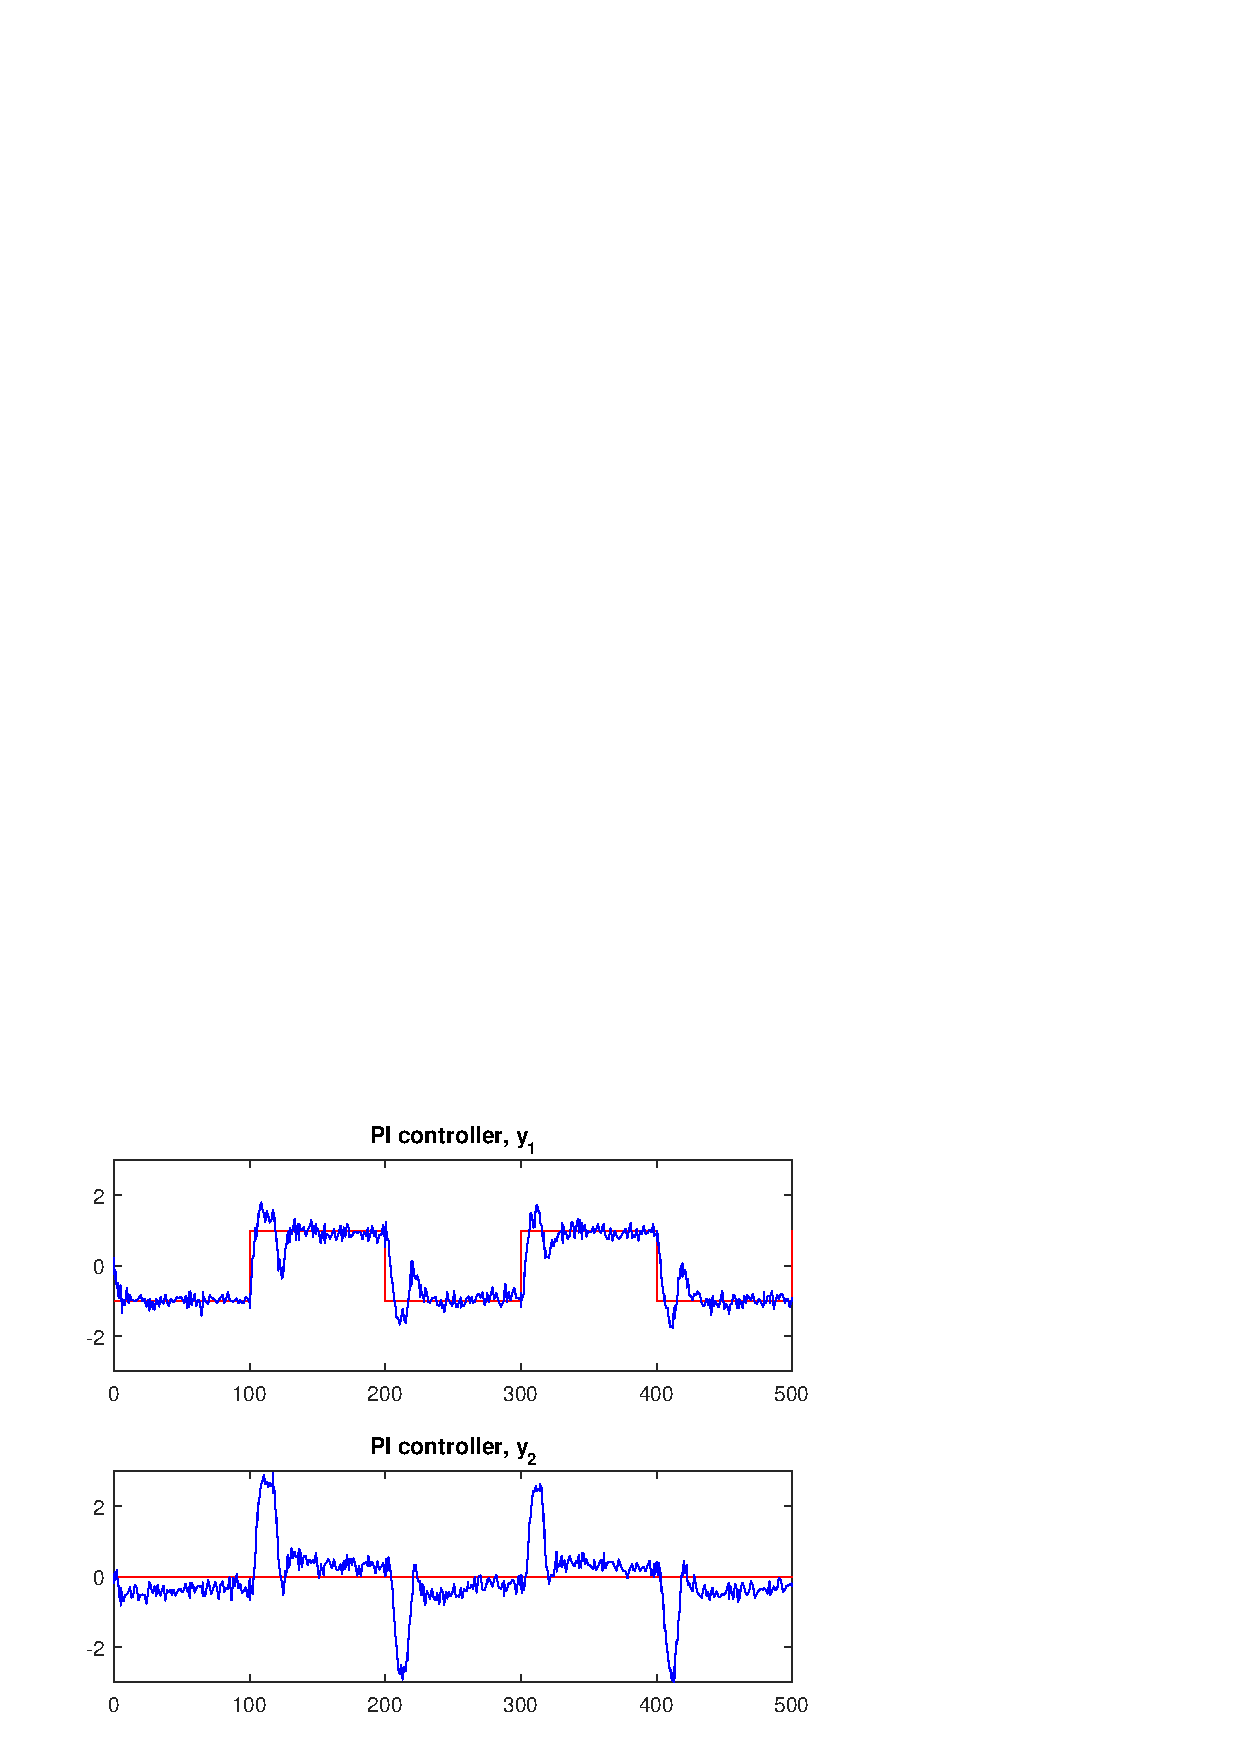
\includegraphics[width=0.8\textwidth]{fig/PI.pdf}
	\caption{PI controller}
	\label{fig:2aPI}
\end{figure}
\begin{figure}[ht!]
	\centering
	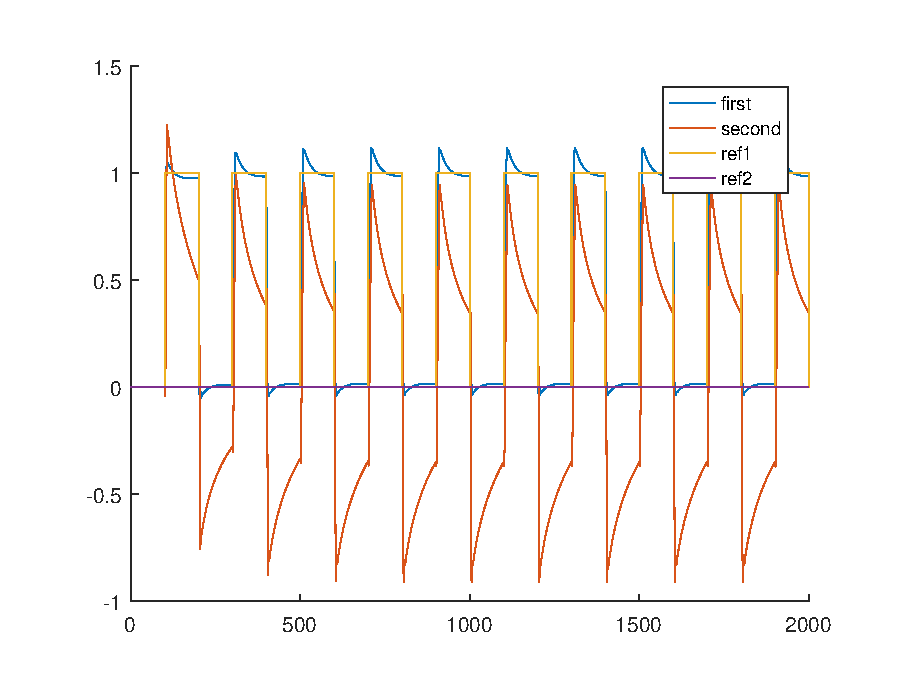
\includegraphics[width=0.8\textwidth]{fig/PI_bad.eps}
	\caption{Bad response from a barely tuneid PI controller}
	\label{fig:2aresp}
\end{figure}


\subsection{Dynamic decoupling}
For a decoupled controller we use
\begin{equation}
	\begin{aligned}
		G(s)_{\text{des}} &= W(s)G(s)\\
		\implies W(s)&= G^{-1}(s)G(s)_{\text{des}}
	\end{aligned}
\end{equation}
where $G(s)_{\text{des}}$ is diagonal with the elements from the diagonal of $G(s)$. With the MATLAB code
\begin{lstlisting}[style = Matlab-editor]
	sys = ss(A,B,C,0);
	G = tf(sys);
	Gdes = blkdiag(G(1,1) , G(2,2));
	W = G\Gdes;
	decoup = ss(W);
\end{lstlisting}
we get a state space model with our new decoupled model added as shown in \autoref{fig:2bdec}.
\begin{figure}[ht!]
	\centering
	\includegraphics[width=0.8\textwidth]{fig/decoupling.pdf}
	\caption{System with decoupled state space model added}
	\label{fig:2bdec}
\end{figure}

Without saturation on the input the system, especially the second output, follows the reference good. This is shown in \autoref{fig:2bunsat}. However when saturation is added we see that are model is wrong as the results are crazy. This is shown in \autoref{fig:2bsat}.
\begin{figure}[ht!]
	\centering
	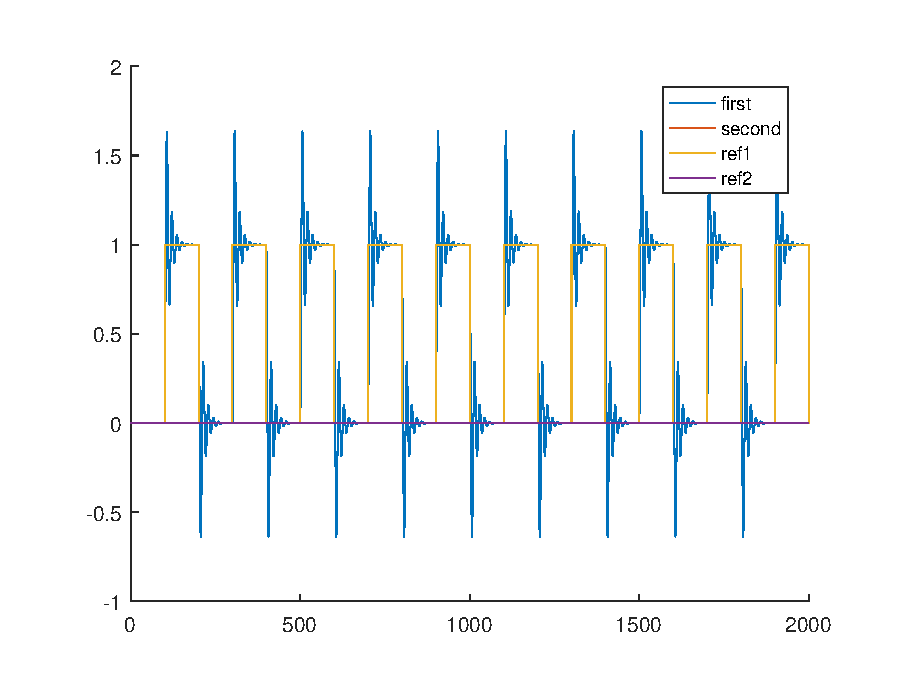
\includegraphics[width=0.8\textwidth]{fig/decoup_unsaturated.eps}
	\caption{Output of the system with decoupling and without saturation on input}
	\label{fig:2bunsat}
\end{figure}
\begin{figure}[ht!]
	\centering
	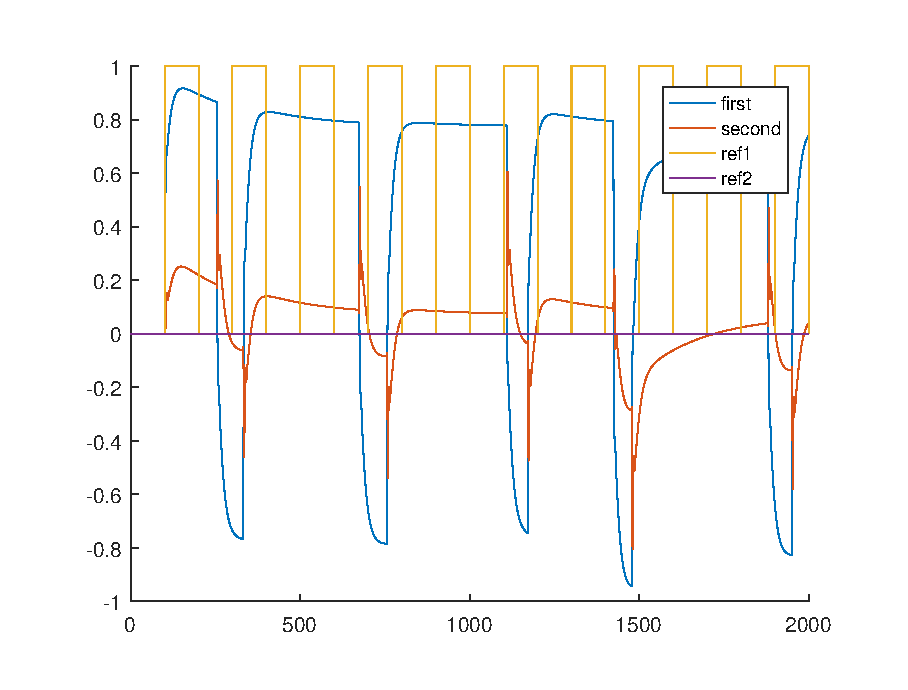
\includegraphics[width=0.8\textwidth]{fig/decoup_saturated.eps}
	\caption{Output of the system with decoupling and saturation on input}
	\label{fig:2bsat}
\end{figure}

\clearpage
\subsection{Kalman filter}
With a Kalman filter added as shown in \autoref{fig:2cKalman} and the MATLAB code 
\begin{lstlisting}[style = Matlab-editor]
	[K,S,e] = lqr(A,B,eye(5), eye(2));
\end{lstlisting}
we get a LQR-controller. Combining this with the PI-controller we could get better results when noise is added to the system, because of the use of state estimatoors instead of noisy measurements.
\begin{figure}[ht!]
	\centering
	\includegraphics[width=0.8\textwidth]{fig/Kalman.pdf}
	\caption{Kalman filter added to PI controller model}
	\label{fig:2cKalman}
\end{figure}

\end{document}